\section{Problema de transporte}

\subsection{Introducción}
En este tema se estudiará el problema del transporte entre ciertos origenes y destinos. La característica común de los
modelos que se estudiarán es que los arrays\footnote{Estructura de datos que almacena una colección de elementos} resultantes 
serán completos, a diferencia de los arrays dispersos que se usarán en los problemas de flujos de redes.

\subsection{Descripción general}

El problema general del transporte se refiere a la distribución de bienes desde $m$ origenes (o centros de abastecimiento)
a $n$ destinos (o puntos de demanda) con el menor coste posible. Cada centro $i=1,\dots,m$ tiene asociado un coeficiente
$s_i$ que representa la oferta (cantidad máxima) que puede suministrar. Asi mismo, a cada punto demanda $j=1,\dots,n$ se
le asocia un coeficiente $d_j$ representando la cantidad requerida en dicho punto. Por último, asociado a cada ``trayectoria''
existe un coeficiente $c_{ij}$ que representa el coste por unidad de bien transportada desde el centro $i$ al punto $j$.

Definidos los coeficientes, el problema de transportes pretende suplir las demandas de los puntos desde los centros 
minimizando el coste total. Por tanto el planteamiento general es el siguiente

\begin{alignat}{3}
    \text{minimizar:}   & \quad & \sum^m_{i=1}\sum^n_{j=1}c_{ij}x_{ij}     & \quad &                        \label{eq:1}\\
    \text{sujeto a:}    & \quad & \sum^n_{j=1}x_{ij}\leq s_i               &       & \forall i=1,\dots,m    \label{eq:2}\\
                        & \quad & \sum^m_{i=1}x_{ij}\geq d_j               &       & \forall j=1,\dots,n    \label{eq:3}\\
                        & \quad & x_{ij}\geq 0                             &       & \forall i,j            \label{eq:4}
\end{alignat}

donde $x_{ij}$ representa la cantidad del bien transportado por la trayectoria que une el centro $i$ con el punto $j$.

\vspace*{2mm}

La función \ref{eq:1} se refiere al coste total del transporte. La restricción enunciada en \ref{eq:2} impide que se 
consuma más que la oferta ofrecida por un centro $i$. La restricción \ref{eq:3} es el equivalente para la demanda. Asegura
que se satisface la demanda en el punto $j$.

\vspace*{2mm}

Se considerará problema de transporte cualquier problema de programación lineal que tenga una forma análoga a la anterior,
sin necesariamente referirse a la distribución de algun bien.

\newpage

Para un problema de transporte se define la oferta total como la suma de las ofertas de cada centro, $O_T=\sum^m_{i=1}s_i$,
y la demanda total como la suma de las demandas de cada punto, $D_T=\sum^n_{j=1}d_j$. Se define un problema como de transporte 
balanceado cuando $O_T=D_T$. En caso de problema balanceado todas las restricciones (salvo la de no negatividad) se cumplen en
forma de igualdad, pudiendose reformular como

\begin{alignat}{3}
    \text{minimizar:}   & \quad & \sum^m_{i=1}\sum^n_{j=1}c_{ij}x_{ij}     & \quad &                        \\
    \text{sujeto a:}    & \quad & \sum^n_{j=1}x_{ij}= s_i                  &       & \forall i=1,\dots,m    \\
                        & \quad & \sum^m_{i=1}x_{ij}= d_j                  &       & \forall j=1,\dots,n    \\
                        & \quad & x_{ij}\geq 0                             &       & \forall i,j            
\end{alignat}

Cuando un problema no está balanceado, es facil convertirlo a uno que si. Cuando la oferta excede a la demanda total se 
añadirá un punto de demanda ficticio con demanda igual a la excedente de la oferta (como los envios a este punto no
se deben tener en cuenta, se asignará un coste 0). Estos puntos de demanda ficticios representan la oferta no usada, asi
pues, son las variables de holgura de las restricciones de oferta.

\noindent En caso de que la demanda sea mayor que la oferta ($D_T<O_T$), el problema no es factible.

\subsection{Obtención de soluciones factibles}

\begin{flushright}
    \textit{En lo que sigue, se consideran siempre problemas balanceados}
\end{flushright}

Un problema de transporte se puede representar en una tabla conocida como \textbf{tabla de transporte}

\begin{center}
    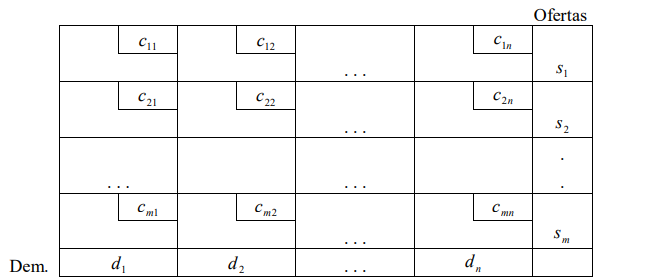
\includegraphics[width=0.9\textwidth]{img/TablaTransporte.png}
\end{center}

Dada una solución factible $X=(x_{1}|\cdots|x_{m})$ el valor asignado a cada variable $x_{ij}$ se sitúa en el interior
de la celda $ij$-ésima de la tabla. Todos los métodos de resoluciín que se ven utilizan esta tabla como base para la
realización de los cálculos. 

\newpage

\begin{itemize}
    \item \textbf{Método de la esquina noroeste}. Partimos de la tabla de transporte y comenzamos con la esquina superior
          izquierda (la que se encuentra más al ``noroeste''). A la variable $x_{11}$ se le asigna el máximo valor posible,
          esto es $min\{s_1, d_1\}$. Si se asigna $s_1$ esto significa que ningún otro punto podrá recibir el bien desde
          el primer centro, por lo que se tachan el resto de celdas de la fila y se sustituye $d_1$ por $d_1-s_1$. De
          forma análoga, si $x_{11}=d_1$ significa que se ha suplido toda la demanda del primer punto, por lo que se tachan
          el resto de celdas de la columna y se actualiza la cantidad de oferta $s_1-d_1$. Se repite el procedimiento 
          eligiendo de nuevo la próxima celda con el ``criterio noroeste'' entre las celdas disponibles (no tachadas) hasta
          que toda la demanda haya sido asignada.
    \item \textbf{Método greedy o de coste mínimo}. El anterior método no tiene en cuenta los costes de las trayectorias, por
          lo que a pesar de proporcionar una solución factible, rara vez se trata de la solución óptima. El procedimiento es
          el mismo pero cambia el criterio de selección de la celda, tomandose en cada iteración la celda de menor coste
          disponible.
    \item \textbf{Método de Vogel}. Para cada fila (columna) se calcula una penalización igual a la diferencia entre los dos 
          costes más pequeños de dicha fila (columna). Esta penalización indica el coste en el que se incurre por no elegir el 
          coste mínimo de dicha fila (columna). Se asigna el criterio de selección de celda a la menor penalización. En cada
          etapa se deben recalcular las penalizaciones. En caso de empate entre penalizaciones, se eligirá la del coste
          mínimo.
\end{itemize}

El método de coste mínimo puede (de casualidad) dar mejores resultados que el resto, pero por lo general el método de Vogel 
es el que genera una solución más cercana a la óptima, encontrando en ocasiones esta misma.

\subsection{Variantes del problema}

El problema de transportes general tiene numerosas variantes (o extensiones). Aquí se listan algunas de ellas

\begin{itemize}
    \item \textbf{Problemas no balanceados}. Ya hemos visto como se pueden formularse con igualdades.
    \item \textbf{Problemas de maximización}. En ocasiones se trata de maximizar una utilidad o un beneficio, siguiendo
          las restricciones típicas del problema de transporte. En este caso los criterios se deben tener en cuenta de 
          forma contraria, es decir, donde antes se buscaba el menor, ahora se busca el mayor.
    \item \textbf{Rutas prohibidas} (grafo no completo). En ocasiones no es posible enviar unidades desde el centro $i$
          al punto $j$. La forma más sencilla es considerar el problema como uno de redes, el cual simplemente elimina
          la variable $x_{ij}$. La segunda posibilidad es considerar el coste de la ``trayectoria'' muy elevado para que la
          variable $x_{ij}$ valga 0. Finalmente, otra tercera posibilidad es añadir la restricción  $x_{ij}=0$.
          \item \textbf{Caso capacitado}. En un problema de transporte con capacidades, se tienen las restricciones de cotas
          superiores para las variables de la forma $0\leq x_{ij}\leq u_{ij}$ para todas las rutas con capacidad. La 
          capacidad limita la cantidad del bien que puede ser enviada por una ``trayectoria'', por lo que se deben añadir
          estas restricciones cuando $u_{ij}<min\{s_i, d_i\}$ (no sería necesario añadirlas en caso contrario, pues ya 
          existen restricciones para $s_i$ y $d_i$).
\end{itemize}

\newpage

\subsection{Transporte Multiproducto}

En ocasiones, desde los centros de oferta, pueden salir distintos bienes o productos que pueden ser requeridos todos o algunos
de ellos desde los puntos de demanda. En este caso aumentan mucho los parámetros que intervienen en el problema. De forma
general consideraremos

\begin{center}
    \begin{tabular}{rcl}
        $m$         & = & número de puntos oferta \\
        $n$         & = & número de puntos demanda \\
        $p$         & = & número de productos ofertados y demandados \\
        $s_i^k$     & = & oferta del producto $k$ en el centro $i$ \\
        $d_j^j$     & = & demanda del producto $k$ en el punto $j$ \\
        $u_{ij}$    & = & cantidad máxima de flujo permitida en la ``trayectoria'' $ij$-ésima \\
        $c_{ij}^k$  & = & coste de transportar una unidad del producto $k$ del centro $i$ al punto $j$ \\
    \end{tabular}
\end{center}

El problema de encontrar la distribución de los productos con el mínimo coste posible se formula de la siguiente forma

\begin{alignat}{5}
    \text{minimizar:}   & \quad & \sum_{i,j,k}c_{ij}^kx_{ij}^k  & \quad &               \\
    \text{sujeto a:}    & \quad & \sum_{jk}x_{ij}^k\leq s_i^k   &       & \forall i,k   \\
                        & \quad & \sum_{ik}x_{ij}^k\leq d_i^k   &       & \forall j,k   \\
                        & \quad & \sum_kx_{ij}^k\leq u_{ij}     &       & \forall i,j   \\
                        & \quad & x_{ij}^k\geq 0                &       & \forall i,j,k           
\end{alignat}

donde $x_{ij}^k$ son las unidades del producto $k$ transportadas del centro $i$ al punto $j$.

\subsection{Transporte Multimodal}

En esta ocasión, pueden haber distintos modos de transporte (camión, tren, barco, \dots). También se puede tratar de 
distintas empresas o transportistas, cada una con su centro de distribución. De forma general (y para el caso de un único
producto) consideramos

\begin{center}
    \begin{tabular}{rcl}
        $m$         & = & número de puntos oferta \\
        $n$         & = & número de puntos demanda \\
        $p$         & = & número de modos de transporte \\
        $s_i$       & = & oferta en el centro $i$ \\
        $d_j$       & = & demanda en el punto $j$ \\
        $u_k$       & = & cantidad máxima que se puede distribuir por el medio de transporte $k$ \\
        $c_{ij}^k$  & = & coste de transportar del centro $i$ al punto $j$ mediante el transporte $k$ \\
    \end{tabular}
\end{center}

\newpage

El problema de encontrar la distribución del producto con el mínimo coste posible se formula de la siguiente forma

\begin{alignat}{5}
    \text{minimizar:}   & \quad & \sum_{i,j,k}c_{ij}^kx_{ij}^k  & \quad &               \\
    \text{sujeto a:}    & \quad & \sum_{jk}x_{ij}^k\leq s_i^k   &       & \forall i     \\
                        & \quad & \sum_{ik}x_{ij}^k\leq d_i^k   &       & \forall j     \\
                        & \quad & \sum_kx_{ij}^k\leq u_k        &       & \forall k     \\
                        & \quad & x_{ij}^k\geq 0                &       & \forall i,j,k           
\end{alignat}

donde $x_{ij}^k$ son las unidades del producto transportadas por el modo $k$ del centro $i$ al punto $j$.

\subsection{Producción-Distribución}

Se considera un problema en el que no solo hay costes de distribución, sino que se añaden los costos de producción, que
pueden ser diferentes en cada origen. Se desea conocer el nivel de producción que satisfaga las demandas sin superar
la capacidad de producción de cada centro y la distribución de la mercancía de forma que los costes totales sean mínimos. De
forma general consideraremos

\begin{center}
    \begin{tabular}{rcl}
        $m$         & = & número de fabricas o centros de producción \\
        $n$         & = & número de puntos demanda \\
        $s_i$       & = & capacidad de producción del centro $i$ \\
        $d_j$       & = & demanda en el punto $j$ \\
        $p_i$       & = & coste por unidad producida en la fabrica $i$ \\
        $u_k$       & = & cantidad máxima de flujo permitida en la ``trayectoria'' $ij$-ésima \\
        $c_{ij}$    & = & coste de transportar del centro $i$ al punto $j$ \\
    \end{tabular}
\end{center}

Si el problema está balanceado, quedará formulado de la siguiente forma

\begin{alignat}{3}
    \text{minimizar:}   & \quad & \sum^m_{i=1}\sum^n_{j=1}(c_{ij}+p_i)x_{ij}    & \quad &                        \\
    \text{sujeto a:}    & \quad & \sum^n_{j=1}x_{ij}= s_i                       &       & \forall i=1,\dots,m    \\
                        & \quad & \sum^m_{i=1}x_{ij}= d_j                       &       & \forall j=1,\dots,n    \\
                        & \quad & 0 \leq x_{ij} \leq u_{ij}                     &       & \forall i,j            
\end{alignat}

Si la oferta supera a la demanda se sustituyen las restricciones por ``menor o igual'' o ``mayor o igual'' teniendose en
cuenta de que las unidades producidas pero no distribuidas contribuyen con un coste igual al de su producción, o al de 
su producción y almacenamiento.

\newpage

\subsection{Dos etapas}

Es una extensión del problema de transporte que aparece frecuentemente. Suele ser necesario que existan almacenamientos
intermedios, que son puntos de transbordo donde no se acumula la mercancia (todo lo que entra sale). En general 
consideraremos

\begin{center}
    \begin{tabular}{rcl}
        $m$         & = & número de puntos oferta \\
        $n$         & = & número de puntos demanda \\
        $p$         & = & número de almacenes intermedios \\
        $s_i^k$     & = & oferta del en el centro $i$ \\
        $d_j^j$     & = & demanda del producto en el punto $j$ \\
        $c_{ik}^1$  & = & coste de transportar del centro de oferta $i$ al almacen $k$ \\
        $c_{ik}^1$  & = & coste de transportar del el almacen $k$ al punto $j$ \\
    \end{tabular}
\end{center}

Es posible modelizarlo de 3 formas distintas. Como un problema de transporte en dos etapas quedará formulado de la siguiente
forma

\begin{alignat}{6}
    \text{minimizar:}   & \quad & \sum^m_{i=1}\sum^n_{j=1}c_{ij}^1x_{ik}^1 + \sum^m_{i=1}\sum^n_{j=1}c_{ij}^2x_{kj}^2 & \quad &                        \\
    \text{sujeto a:}    & \quad & \sum^p_{k=1}x_{ik}^1\leq s_i  &               & \forall i=1,\dots,m           \\
                        & \quad & \sum^p_{k=1}x_{kj}^2\geq d_j  &               & \forall j=1,\dots,n           \\
                        & \quad & \sum^m_{i=1}x_{ik}^1 = \sum^n{j=1}x_{kj}^2    &       & \forall k=1,\dots,p   \\
                        & \quad & 0 \leq x_{ik}^1                               &       & \forall i,k           \\
                        & \quad & 0 \leq x_{kj}^2                               &       & \forall k,j
\end{alignat}

Como un problema de programación lineal con 3 índices

\begin{alignat}{3}
    \text{minimizar:}   & \quad & \sum^m_{i=1}\sum^p_{k=1}\sum^n_{j=1}(c_{ik}^1 + c_{kj}^2)x_{ikj}  & \quad &   \\
    \text{sujeto a:}    & \quad & \sum^p_{k=1}\sum^n_{j=1}x_{ikj}\leq s_i   &      & \forall i=1,\dots,m1       \\
    \text{sujeto a:}    & \quad & \sum^m_{i=1}\sum^p_{k=1}x_{ikj}\geq d_i   &      & \forall j=1,\dots,m        \\
                        & \quad & 0 \leq x_{ikj}                            &      & \forall i,k,j              \\
\end{alignat}

O como un progema de flujo en redes, que se verá en el proximo capitulo.

\vspace*{5mm}

\noindent Por supuesto, una restricción que se puede añadir en todos los anteriores ejemplos de formulación es la de 
capacidad de los almacenes $u_k$.